\documentclass[english,floatsintext,man]{apa6}

\usepackage{amssymb,amsmath}
\usepackage{ifxetex,ifluatex}
\usepackage{fixltx2e} % provides \textsubscript
\ifnum 0\ifxetex 1\fi\ifluatex 1\fi=0 % if pdftex
  \usepackage[T1]{fontenc}
  \usepackage[utf8]{inputenc}
\else % if luatex or xelatex
  \ifxetex
    \usepackage{mathspec}
    \usepackage{xltxtra,xunicode}
  \else
    \usepackage{fontspec}
  \fi
  \defaultfontfeatures{Mapping=tex-text,Scale=MatchLowercase}
  \newcommand{\euro}{€}
\fi
% use upquote if available, for straight quotes in verbatim environments
\IfFileExists{upquote.sty}{\usepackage{upquote}}{}
% use microtype if available
\IfFileExists{microtype.sty}{\usepackage{microtype}}{}

% Table formatting
\usepackage{longtable, booktabs}
\usepackage{lscape}
% \usepackage[counterclockwise]{rotating}   % Landscape page setup for large tables
\usepackage{multirow}		% Table styling
\usepackage{tabularx}		% Control Column width
\usepackage[flushleft]{threeparttable}	% Allows for three part tables with a specified notes section
\usepackage{threeparttablex}            % Lets threeparttable work with longtable

% Create new environments so endfloat can handle them
% \newenvironment{ltable}
%   {\begin{landscape}\begin{center}\begin{threeparttable}}
%   {\end{threeparttable}\end{center}\end{landscape}}

\newenvironment{lltable}
  {\begin{landscape}\begin{center}\begin{ThreePartTable}}
  {\end{ThreePartTable}\end{center}\end{landscape}}




% The following enables adjusting longtable caption width to table width
% Solution found at http://golatex.de/longtable-mit-caption-so-breit-wie-die-tabelle-t15767.html
\makeatletter
\newcommand\LastLTentrywidth{1em}
\newlength\longtablewidth
\setlength{\longtablewidth}{1in}
\newcommand\getlongtablewidth{%
 \begingroup
  \ifcsname LT@\roman{LT@tables}\endcsname
  \global\longtablewidth=0pt
  \renewcommand\LT@entry[2]{\global\advance\longtablewidth by ##2\relax\gdef\LastLTentrywidth{##2}}%
  \@nameuse{LT@\roman{LT@tables}}%
  \fi
\endgroup}


  \usepackage{graphicx}
  \makeatletter
  \def\maxwidth{\ifdim\Gin@nat@width>\linewidth\linewidth\else\Gin@nat@width\fi}
  \def\maxheight{\ifdim\Gin@nat@height>\textheight\textheight\else\Gin@nat@height\fi}
  \makeatother
  % Scale images if necessary, so that they will not overflow the page
  % margins by default, and it is still possible to overwrite the defaults
  % using explicit options in \includegraphics[width, height, ...]{}
  \setkeys{Gin}{width=\maxwidth,height=\maxheight,keepaspectratio}
\ifxetex
  \usepackage[setpagesize=false, % page size defined by xetex
              unicode=false, % unicode breaks when used with xetex
              xetex]{hyperref}
\else
  \usepackage[unicode=true]{hyperref}
\fi
\hypersetup{breaklinks=true,
            pdfauthor={},
            pdftitle={Many Labs 5: Registered multisite replication of tempting-fate effects in Risen \& Gilovich (2008)},
            colorlinks=true,
            citecolor=blue,
            urlcolor=blue,
            linkcolor=black,
            pdfborder={0 0 0}}
\urlstyle{same}  % don't use monospace font for urls

\setlength{\parindent}{0pt}
%\setlength{\parskip}{0pt plus 0pt minus 0pt}

\setlength{\emergencystretch}{3em}  % prevent overfull lines

\ifxetex
  \usepackage{polyglossia}
  \setmainlanguage{}
\else
  \usepackage[english]{babel}
\fi

% Manuscript styling
\captionsetup{font=singlespacing,justification=justified}
\usepackage{csquotes}
\usepackage{upgreek}

 % Line numbering
  \usepackage{lineno}
  \linenumbers


\usepackage{tikz} % Variable definition to generate author note

% fix for \tightlist problem in pandoc 1.14
\providecommand{\tightlist}{%
  \setlength{\itemsep}{0pt}\setlength{\parskip}{0pt}}

% Essential manuscript parts
  \title{Many Labs 5: Registered multisite replication of tempting-fate effects
in Risen \& Gilovich (2008)}

  \shorttitle{Multisite replication of tempting fate}


  \author{Maya B. Mathur\textsuperscript{1,2}, Diane-Jo Bart-Plange\textsuperscript{3}, Balazs Aczel\textsuperscript{4}, Michael H. Bernstein\textsuperscript{5}, Antonia Ciunci\textsuperscript{5}, Charles R. Ebersole\textsuperscript{3}, Filipe Falcão\textsuperscript{6}, Kayla Gerken\textsuperscript{7}, Rias A. Hilliard\textsuperscript{7}, Alan Jern\textsuperscript{7}, Danielle Kellier\textsuperscript{2}, Grecia Kessinger\textsuperscript{8}, Vanessa Kolb\textsuperscript{5}, Marton Kovacs\textsuperscript{4}, Caio Lage\textsuperscript{9}, Eleanor V. Langford\textsuperscript{3}, Samuel Lins\textsuperscript{6}, Dylan Manfredi\textsuperscript{10}, Venus Meyet\textsuperscript{8}, Don A. Moore\textsuperscript{11}, Gideon Nave\textsuperscript{10}, Christian Nunnally\textsuperscript{7}, Anna Palinkas\textsuperscript{4}, Kimberly P. Parks\textsuperscript{3}, Sebastiaan Pessers\textsuperscript{12}, Tiago Ramos\textsuperscript{6}, Kaylis Hase Rudy\textsuperscript{8}, Janos Salamon\textsuperscript{4}, Rachel L. Shubella\textsuperscript{7}, Rúben Silva\textsuperscript{6}, Sara Steegen\textsuperscript{12}, L.A.R. Stein\textsuperscript{5,13,14}, Barnabas Szaszi\textsuperscript{4}, Peter Szecsi\textsuperscript{4}, Francis Tuerlinckx\textsuperscript{12}, Wolf Vanpaemel\textsuperscript{12}, Maria Vlachou\textsuperscript{12}, Bradford J. Wiggins\textsuperscript{8}, David Zealley\textsuperscript{8}, Mark Zrubka\textsuperscript{4}, \& Michael C. Frank\textsuperscript{2}}

  \def\affdep{{"", "", "", "", "", "", "", "", "", "", "", "", "", "", "", "", "", "", "", "", "", "", "", "", "", "", "", "", "", "", "", "", "", "", "", "", "", "", "", "", ""}}%
  \def\affcity{{"", "", "", "", "", "", "", "", "", "", "", "", "", "", "", "", "", "", "", "", "", "", "", "", "", "", "", "", "", "", "", "", "", "", "", "", "", "", "", "", ""}}%

  \affiliation{
    \vspace{0.5cm}
          \textsuperscript{1} Harvard University, Boston, MA, United States\\
          \textsuperscript{2} Stanford University, Stanford, CA, United States\\
          \textsuperscript{3} University of Virginia, Charlottesville, VA, United States\\
          \textsuperscript{4} ELTE Eötvös Loránd University, Budapest, Hungary\\
          \textsuperscript{5} University of Rhode Island, Kingston, RI, United States\\
          \textsuperscript{6} University of Porto, Porto, Portugal\\
          \textsuperscript{7} Rose-Hulman Institute of Technology, Terre Haute, IN, United States\\
          \textsuperscript{8} Brigham Young University - Idaho, Rexburg, ID, United States\\
          \textsuperscript{9} Pontifical Catholic University of Rio de Janeiro, Rio de Janeiro, Brazil\\
          \textsuperscript{10} University of Pennsylvania, Philadelphia, PA, United States\\
          \textsuperscript{11} University of California at Berkeley, Berkeley, CA, United States\\
          \textsuperscript{12} University of Leuven, Belgium\\
          \textsuperscript{13} Brown University, Providence, RI, United States\\
          \textsuperscript{14} Rhode Island Training School, Cranston, RI, United States  }

 % If no author_note is defined give only author information if available
      \newcounter{author}
                              \authornote{
            Correspondence concerning this article should be addressed to Maya B. Mathur, Quantitative Sciences Unit, 1070 Arastradero Rd, Palo Alto, CA, 94305. E-mail: \href{mailto:mmathur@stanford.edu}{\nolinkurl{mmathur@stanford.edu}}
          }
                                                                                                                                                                                                                                                                                                                                                                                                                                                                                                                                                                                                    

  \abstract{Risen \& Gilovich (2008) found that subjects believe that ``tempting
fate'' will be punished with ironic bad outcomes (a main effect) and
that this effect is magnified under cognitive load (an interaction). A
previous replication project (Open Science Collaboration, 2015) failed
to replicate both the main effect and the interaction in an online
implementation of the protocol that used Amazon Mechanical Turk. Before
this replication was run, the authors of the original study expressed
concern that the cognitive load manipulation may be less effective when
implemented online and that subjects recruited online may respond
differently to the specific experimental scenario chosen for
replication. A later, large replication project (Many Labs 2) replicated
the main effect (though the effect size was smaller than in the original
study), but did not test for an interaction. To attempt to replicate the
interaction while addressing the original authors' concerns regarding
the 2015 protocol, we developed a new protocol in collaboration with the
original authors. We used 4 university sites (\(n=XXX\) total) chosen
for similarity to the site of the original study to conduct a
high-powered, preregistered replication focused primarily on the
interaction effect. Results {[}supported/did not support{]} the focus
interaction or the main effect and were {[}more pronounced/less
pronounced/comparable{]} in 6 additional universities that were less
similar to the original site. Post hoc analyses {[}provided/did not
provide{]} strong evidence for statistical inconsistency between the
original study's estimates and the replications; that is, the original
study's results {[}would/would not{]} have been {[}extremely
unlikely/unlikely/likely/extremely likely{]} in the estimated
distribution of the replications. We also collected a new Mechanical
Turk sample under the previous replication protocol, indicating that the
updated protocol (i.e., conducting the study in person and in
universities similar to the original site) {[}did not meaningfully
change replication results/yielded replications results more similar to
the original study{]}. Secondary analyses {[}supported/failed to
support{]} substantive mechanisms for the failure to replicate.}
  \keywords{replication, reproducibility, preregistered, open data, heuristic,
magical thinking \\

    
  }




  \usepackage{caption}

\usepackage{amsthm}
\newtheorem{theorem}{Theorem}
\newtheorem{lemma}{Lemma}
\theoremstyle{definition}
\newtheorem{definition}{Definition}
\newtheorem{corollary}{Corollary}
\newtheorem{proposition}{Proposition}
\theoremstyle{definition}
\newtheorem{example}{Example}
\theoremstyle{definition}
\newtheorem{exercise}{Exercise}
\theoremstyle{remark}
\newtheorem*{remark}{Remark}
\newtheorem*{solution}{Solution}
\begin{document}

\maketitle

\setcounter{secnumdepth}{0}



\captionsetup[table]{labelformat=empty}
\captionsetup[figure]{labelformat=empty}

Risen and Gilovich (2008) examined the existence and mechanisms of the
belief that \enquote{tempting fate} is punished with ironic bad
outcomes. They hypothesized, for example, that students believe that
they are more likely to be called on in class to answer a question about
the assigned reading if, in fact, they had not done the reading (and
thus had \enquote{tempted fate}) versus if they had come to class
prepared (and thus had not \enquote{tempted fate}). Risen and Gilovich
(2008) additionally hypothesized that deliberative thinking (sometimes
termed \enquote{System 2} processing (Epstein, Lipson, Holstein, \& Huh,
1992)) may help suppress irrational heuristics regarding tempting fate,
and thus a cognitive load manipulation designed to preoccupy System 2
resources would magnify the effect of tempting fate on subjects'
perceived likelihood of a bad outcome. That is, they hypothesized a
positive interaction between cognitive load and tempting fate on
subjects' perceived likelihood of an ironic bad outcome.

Risen and Gilovich (2008)'s Study 6, the focus of replication, used a
between-subjects factorial design to assess this possibility (total
analyzed \(n=120\)). Subjects were randomly assigned to read a scenario
in which they imagined themselves having tempted fate by not having done
the assigned reading or, alternatively, not having tempted fate by
having done the assigned reading. Additionally, subjects were randomly
assigned to complete the task with or without cognitive load. Subjects
not under cognitive load simply read the scenario and then judged the
likelihood of being called on in class. Subjects under cognitive load
counted backwards by 3s from a large number while reading the scenario,
after which they provided the likelihood judgment. This study provided
evidence for the predicted main effect of tempting fate in subjects not
assigned to cognitive load (estimated difference in perceived likelihood
on a 0-10 scale after tempting fate vs.~not tempting fate: \(b=\) 1.03
with 95\% CI: {[}0.09, 1.97{]}; \(p=\) 0.03)\footnote{Approximate effect
  sizes were recomputed from rounded values in Risen and Gilovich
  (2008).} as well as the focus interaction effect (estimated effect of
tempting fate vs.~not tempting fate for subjects under cognitive load
vs.~not under cognitive load: \(b=\) 1.54 with 95\% CI: {[}0.05,
3.03{]}; \(p=\) 0.04).

We selected Risen and Gilovich (2008) for replication because, per the
selection criteria of all Many Labs 5 replications, this study was
subject to a previous replication attempt by Open Science Collaboration
(2015). The previous replication found little evidence for either a main
effect of tempting fate without cognitive load (\(n=226\), \(b=\) 0.20
with 95\% CI: {[}-0.58, 0.97{]}; \(p=\) 0.62) or the focus interaction
(\(b=\) 0.03 with 95\% CI: {[}-1.14, 1.20{]}; \(p=\) 0.96) (Mathur \&
Frank, 2012). However, prior to the collection of replication data by
this previous replication effort (termed \enquote{RPP}), the authors of
the original study expressed concerns about the replication protocol.
Due to feasibility constraints, the RPP replication proceeded without
addressing these concerns. Specifically, the replication was implemented
on the crowdsourcing website Amazon Mechanical Turk, a setting that
could potentially compromise the cognitive load manipulation if subjects
were already multitasking or were distracted. Additionally, the
experimental scenario, which required subjects to imagine being
unprepared to answer questions in class, may be less personally salient
to subjects not enrolled in an elite university similar to Cornell
University, the site of the original study. Thus, as part of the Many
Labs 5 project, the present multisite replication aimed to: (1) reassess
replicability of Risen and Gilovich (2008) using an updated protocol
designed in collaboration with the original authors to mitigate
potential problems with the previous replication protocol; and (2)
formally assess the effect of updating the protocol in this manner by
comparing its results to newly collected results under the previous
replication protocol.

Concurrently with the present study, an independent group (Many Labs 2,
or \enquote{ML2}) conducted a multisite replication of the main effect,
but not the interaction (Klein, 2017). Their primary analysis sample
comprised undergraduates at universities and colleges in the United
States and abroad (\(n=4599\)). These subjects judged the likelihood of
being called on to be higher when they had tempted fate (mean = 4.61, SD
=2.42) than when they had not tempted fate (mean = 4.07, SD = 2.36;
\(t\)(4,597) =7.57, \(p\) = 4.4e-14, \(d\) = 0.22, 95\% CI
\([0.17, 0.28]\)), providing strong evidence for a main effect of
tempting fate, albeit of smaller magnitude than in the original study.
We discuss the results of the present study in light of these existing
findings.

\section{Disclosures}\label{disclosures}

The protocol, sample size criteria, exclusion criteria, and statistical
analysis plan were preregistered\footnote{One site (BYUI) was permitted
  to collect data prior to preregistration of the statistical analysis
  plan due to their time constraints; the lead investigator and all
  other authors remained blinded to this site's results until
  preregistration and data collection were complete.} with details
publicly available (\href{}{https://osf.io/8y6st/} for the protocol and
XXX for the analyses); departures from these plans are reported in this
manuscript. All data, materials, and analysis code are publicly
available and documented (XXX). Sites obtained ethics committee approval
when appropriate to their geographical location and institutional
requirements, and data were collected in accordance with the Declaration
of Helsinki.

\section{Methods}\label{methods}

In consultation with the original authors, we designed a replication
procotol that more closely duplicated the original design than did the
RPP replication (Table 1). Primary analyses used only data from
university sites located in the United States and meeting an academic
criterion for similarity to the original site (Table 1, row 1); these
sites are termed \enquote{similar sites}. We additionally used the
previous RPP replication protocol without modification to collect a new
sample on Amazon Mechanical Turk (\enquote{MTurk}). Finally, we
collected secondary data in several universities not meeting the SAT
criterion for similarity to Cornell or located outside the United
States, henceforth termed \enquote{dissimilar sites}. Data from
dissimilar sites were used in secondary analyses to further increase
power and assess whether, as hypothesized, site similarity in fact
moderates the focus effect. For sites whose subjects were not expected
to speak fluent English, questionnaire materials were translated and
verified through independent back-translation.

\begin{figure}
\centering
\includegraphics{summary_table/table_1.png}
\caption{Table 1: Comparison of experimental protocols used in the
original study, the RPP replication, and the present replication.}
\end{figure}

The primary statistical estimands were (1) the focus interaction within
similar sites and (2) the difference in this interaction between similar
sites and MTurk (modeled as a three-way interaction, as described
below). Sample sizes were chosen to provide, in aggregate, more than
80\% power to detect a three-way interaction with effect size more than
\(0.75\) standard deviations of perceived likelihood. Because detecting
the three-way interaction requires substantially larger sample sizes
than detecting the focus interaction alone, this choice of sample sizes
also provided \(>99\%\) power to detect, within similar sites alone, a
focus interaction of the size reported in the original study. Each site
additionally attempted to reach these power criteria internally, though
in many cases this was not feasible. Site-level and aggregate analyses
were conducted by one author (MBM), who was blinded to results until all
sites had completed data collection; these analyses were audited for
accuracy by other authors.

We collected four new measures, developed in discussion with the
original authors, for use in secondary analyses. As manipulation checks
for the effectiveness of the cognitive load manipulation, we asked
subjects assigned to cognitive load to assess on a 0-10 scale the
perceived effort associated with this task (\emph{\enquote{How much
effort did the counting task require?}}) and the task's difficulty
(\emph{\enquote{How difficult was the counting task?}}). Additionally,
the original authors speculated that the experimental scenario
(regarding answering questions in class) may be personally salient to
subjects in an academically competitive environment similar to the site
of the original study, but may be less so for MTurk subjects or subjects
in dissimilar universities. To assess this possibility, we developed new
measures in collaboration with the original authors which required
subjects to evaluate on a 0-10 scale the importance of answering
questions correctly in class (\emph{\enquote{If you were a student in
the scenario you just read about, how important would it be for you to
answer questions correctly in class?}}) and the perceived negativity of
answering incorrectly (\emph{\enquote{If you were a student in the
class, how bad would you feel if you were called on by the professor,
but couldn't answer the question?}}).

\section{Results}\label{results}

\subsection{Descriptive analyses}\label{descriptive-analyses}

Table 2 displays sample sizes, the number of exclusions, and protocol
characteristics for all sites. To estimate the main effect of tempting
fate and the focus interaction within each site, we fit an ordinary
least squares regression model of perceived likelihood on tempting fate,
cognitive load, and their interaction within each site. This analysis
approach is statistically equivalent to the ANOVA model fit in the
original study while also yielding coefficient estimates that are
directly comparable to those estimated in primary analysis models,
discussed below. Figures 1 and 2, respectively, display these
within-site estimates for the main effect and interaction.\footnote{An
  alternative for the study-specific estimates would be to use estimates
  of random intercepts and random slopes by site from the mixed model,
  but here we use subset analyses for a descriptive characterization
  that relaxes the across-site distributional assumptions of the mixed
  model.}

\begin{figure}
\centering
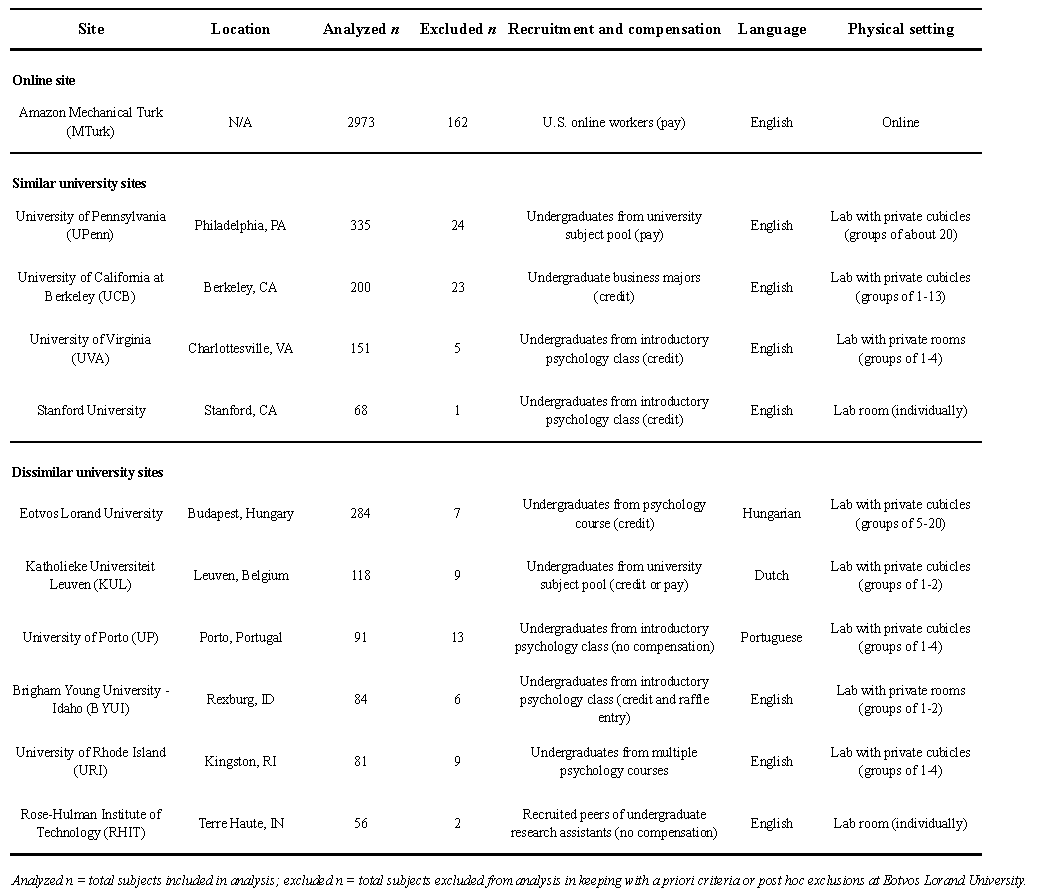
\includegraphics{summary_table/table_2.pdf}
\caption{Table 2: Summary of sites and participants.}
\end{figure}

Among the 4 similar sites, XXX had main effect estimates in the same
direction as the original study estimate, {[}comment on their relative
effect sizes{]}. Main effect estimates in similar sites had \(p\)-values
ranging from XXX to XXX. In the MTurk sample, the main effect estimate
was {[}in the same direction as/in the opposite direction from{]} the
original, {[}comment on its effect size compared to original{]}, and it
was {[}larger than/smaller than/nearly identical to{]} the estimate
previously obtained under the same protocol in RPP. Considering all 10
university sites, XXX had main effect estimates in the same direction as
the original study. These estimates were {[}of smaller magnitude than/of
larger magnitude than/of similar magnitude to{]} the original estimate.

{[}Insert forest plot for main effect estimates ordered by site type
(MTurk, similar, dissimilar) and then by sample size. Legend: Point
estimates and 95\% CIs for each site (black circles) are from ordinary
least squares regression fit to that site's data. For similar sites,
pooled point estimates and 95\% CIs (orange diamonds) are from the
primary mixed model. For dissimilar sites (orange diamonds), these are
from the secondary mixed model. Pooled point estimates represent the
average main effect among subjects in similar universities or in all
universities.{]}

Considering the focus interaction estimate, XXX of 4 similar sites had
estimates in the same direction as the original, and these were {[}of
similar magnitude/of larger magnitude/of smaller magnitude{]} with
\(p\)-values ranging from XXX to XXX. In the MTurk sample, the
interaction estimate was in the {[}same/opposite{]} direction from the
original estimate and was {[}similar/larger/smaller{]} in magnitude
{[}than/to{]} the RPP estimate. Considering all 10 university sites, XXX
had point estimates in the same direction as the original study,
{[}comment on their relative magnitudes compared to original{]}.
\(p\)-values across all universities ranged from XXX to XXX. {[}note if
any sites were outliers{]}

{[}Insert forest plot for interaction estimates ordered by site type
(MTurk, similar, dissimilar) and then by sample size. Legend: Point
estimates and 95\% CIs for each site (black circles) are from ordinary
least squares regression fit to that site's data. For similar sites,
pooled point estimates and 95\% CIs (orange diamonds) are from the
primary mixed model. For dissimilar sites (orange diamonds), these are
from the secondary mixed model. Pooled point estimates represent the
average interaction effect among subjects in similar universities or in
all universities.{]}

\subsection{Primary analyses}\label{primary-analyses}

Primary analyses aimed to: (1) estimate the focus interaction and the
main effect under the updated protocol in similar sites; and (2) assess
whether the focus interaction and the main effect estimates differed
between the updated protocol and the RPP protocol. To this end, we
combined data from the similar sites and MTurk to fit a linear mixed
model with fixed effects representing main effects of tempting fate,
cognitive load, and protocol (similar sites under the updated protocol
vs.~MTurk). To account for correlation of observations within a site,
the model also contained random intercepts by site and random slopes by
site of tempting fate, cognitive load, and their interaction; in all
analyses, all random effects were assumed independently and identically
normal.\footnote{As a planned sensitivity analysis, we also refit the
  same ANOVA model used in the original study, which ignores correlation
  of observations within sites. {[}comment on whether results of this
  analysis were similar to primary results{]} (Supplement). We obtained
  {[}similar/different{]} results in additional sensitivity analyses in
  which we fit a model to only the subset of data from similar sites
  (dropping the MTurk coefficient) or in which we fit meta-analytic
  counterparts to the primary model (Supplement). {[}if relevant,
  comment on how results differed{]}} This model allows estimation of
the focus effect within similar sites and within MTurk and permits
formal assessment of the extent to which these effects differ (via the
three-way interaction of protocol, tempting fate, and cognitive load).
Details of the model specification and interpretations for each
coefficient of interest are provided in the preregistered protocol.

\begin{table}[tbp]
\begin{center}
\begin{threeparttable}
\caption{\label{tab:unnamed-chunk-2}Table 3: In units of perceived likelihood on a 0-10 scale, estimates of the main effect and focus interaction effect in similar university sites and under the RPP protocol (MTurk), as well as estimates of the difference between these estimates. Total n = XXX.}
\begin{tabular}{llll}
\toprule
Parameter & Estimate & 95\% CI & p-value\\
\midrule
Tempt main effect within MTurk & 0.21 & [-0.01, 0.43] & 0.06\\
Tempt main effect within similar sites & 0.11 & [-0.34, 0.56] & 0.64\\
Effect of similar site vs. MTurk on tempt main effect & -0.11 & [-0.61, 0.39] & 0.68\\
Tempt-load interaction within MTurk & -0.20 & [-0.53, 0.13] & 0.24\\
Tempt-load interaction within similar sites & -0.02 & [-0.68, 0.63] & 0.94\\
Effect of similar site vs. MTurk on tempt-load interaction & 0.18 & [-0.56, 0.91] & 0.64\\
\bottomrule
\end{tabular}
\end{threeparttable}
\end{center}
\end{table}

The primary analysis model included XXX subjects from similar sites and
MTurk. Consistent with the RPP replication, the present results
collected on MTurk did not strongly support the main effect of tempting
fate (Table 3), and nor did results collected under the updated protocol
in similar sites (Table 3, row 2). Updating the protocol {[}appeared to
increase/appeared to decrease/did not appear to change{]} the main
effect estimate (Table 3, row 3). Furthermore, results from the new
MTurk sample {[}supported/did not support{]} the focus interaction
(Table 3, row 4), and {[}so did/nor did{]} results under the updated
protocol (Table 3, row 5). Updating the protocol {[}appeared to
increase/appeared to decrease/did not meaningfully affect{]} the focus
interaction estimate (Table 3, row 6). {[}comment on amount of
statistical heterogeneity across sites for both the main effect and
interaction{]}

\subsection{Secondary analyses: All university
sites}\label{secondary-analyses-all-university-sites}

Planned secondary analyses addressed the same questions as the primary
analyses, but additionally incorporated data from dissimilar university
sites (total \(n=\) XXX). Site type was treated as a categorical
variable (MTurk, similar university site, or dissimilar university
site)\footnote{An alternative model specification in which all
  universities were treated as a single category yielded similar results
  (Supplement).}. Additionally, these analyses formally estimated the
difference in results between similar and dissimilar sites. Results
(Table 4) {[}supported/did not support{]} the main effect or the focus
interaction in {[}comment on differences between site types{]}. The main
effect estimate in dissimilar sites was {[}larger than/smaller
than/comparable to{]} that in similar sites (Table 4, row 4),
{[}but/and{]} {[}the interaction estimate was smaller than the original
estimate/the interaction estimate was larger than the original
estimate/as was the interaction estimate{]} (Table 4, row 8). {[}comment
on amount of statistical heterogeneity across sites for both the main
effect and interaction{]} We conducted post hoc secondary analyses
(Supplement) to assess the extent to which the replication findings were
statistically consistent with the original study; that is, whether it is
plausible that the original study was drawn from the same distribution
as the replications (Mathur \& VanderWeele, 2017).

\begin{table}[tbp]
\begin{center}
\begin{threeparttable}
\caption{\label{tab:unnamed-chunk-3}Table 4: In units of perceived likelihood on a 0-10 scale, estimates of the main effect and focus interaction effect in similar university sites, dissimilar university sites, and under the RPP protocol (MTurk), as well as estimates of the difference between these estimates. Total n = XXX.}
\begin{tabular}{llll}
\toprule
Parameter & Estimate & 95\% CI & p-value\\
\midrule
Tempt main effect within MTurk & 0.21 & [-0.22, 0.65] & 0.34\\
Tempt main effect within similar sites & 0.08 & [-0.40, 0.57] & 0.73\\
Tempt main effect within dissimilar sites & 0.42 & [-0.07, 0.90] & 0.09\\
Effect of similar vs. dissimilar site on tempt main effect & -0.33 & [-1.02, 0.36] & 0.35\\
Tempt-load interaction within MTurk & -0.20 & [-1.00, 0.60] & 0.62\\
Tempt-load interaction within similar sites & 0.01 & [-0.73, 0.76] & 0.97\\
Tempt-load interaction within dissimilar sites & -0.28 & [-1.01, 0.45] & 0.45\\
Effect of similar vs. dissimilar site on tempt-load interaction & 0.29 & [-0.75, 1.34] & 0.58\\
\bottomrule
\end{tabular}
\end{threeparttable}
\end{center}
\end{table}

\subsection{Evaluating proposed explanations for replication
failure}\label{evaluating-proposed-explanations-for-replication-failure}

Anticipating that results may have differed between similar and
dissimilar sites, we planned to conduct secondary analyses assessing
proposed explanations for the previous replication failure in RPP.
{[}describe results of secondary analyses assessing whether efficacy of
cognitive load manipulation, perceived effort, or perceived difficulty
differed between MTurk vs.~all university subjects{]}

To assess differences in academic attitudes, we used subjects\footnote{These
  analyses again excluded subjects from UC Berkeley, which did not
  collect the new measures due to a data collection error.} from all
types of sites, including MTurk, to fit linear mixed models regressing
perceived importance (\(n=\) XXX) and perceived negativity (\(n=\) XXX)
on site type (similar, dissimilar, or MTurk) with random intercepts by
site. {[}Supporting/Contrary to{]} our speculation, MTurk subjects
reported that answering questions correctly was {[}less important than
did/as important as/more important than did{]} subjects at similar
universities (\(b=\) XXX with 95\% CI: XXX; \(p=\) XXX) or at dissimilar
universities (\(b=\) XXX with 95\% CI: XXX). Additionally, when asked to
assess how bad it would be to answer incorrectly, MTurk subjects
{[}responded higher than/responded comparably to/responded lower than{]}
subjects at similar sites (\(b=\) XXX with 95\% CI: XXX; \(p=\) XXX) and
at dissimilar sites (\(b=\) XXX with 95\% CI: XXX; \(p=\) XXX).
{[}comment on direction and strength of effects if present{]}

Lastly, in a planned analysis, we assessed variation in results
according to a site's similarity to Cornell, now redefining similarity
using a continuous proxy (namely, a university's estimated median total
SAT score in 2018) rather than the dichotomous \enquote{similar} versus
\enquote{dissimilar} eligibility criterion for primary analyses.
Subjects from universities outside the United States or from MTurk were
excluded from this analysis, leaving an analyzed \(n = XXX\) from 7
universities with median SAT scores ranging from XXX to XXX of 2400
possible points. We assumed that universities with higher SAT scores
would be most similar to Cornell (median SAT: 2134) and therefore
considered a linear effect of median SAT score as a moderator of the
main effects and interaction of tempting fate with cognitive load. A
mixed model {[}suggested/did not suggest{]} that median SAT score
moderated the main effect of tempting fate (\(b=\) XXX for a 10-point
increase in SAT score with 95\% CI: XXX; \(p=\) XXX) or the focus
interaction (\(b=\) XXX with 95\% CI: XXX; \(p=\) XXX`). {[}comment on
direction and strength of interaction if present{]}

\section{Comparison to results of Many Labs
2}\label{comparison-to-results-of-many-labs-2}

{[}Comment on whether results for the main effect were similar to or
different from the findings in Many Labs 2. If similar, no further
analysis needed. If different, compare protocols and analysis approaches
between the two studies in detail and, if possible, attempt follow-up
analyses (flagged as post-hoc) to clarify the extent to which any
protocol differences could account for the discrepancies. Regardless of
whether the main effect appears to replicate in the present study, we
will test for the interaction because, for example, it is possible that
there was a meaningful interaction without a main effect (e.g., the
tempting-fate manipulation \emph{only} affected likelihood judgments in
the cognitive load condition), and this would still partially support
the original study's findings. If our findings do not provide evidence
for the main effect and post hoc analyses identify protocol differences
from ML2 that do appear to account this discrepancy, then, if possible
given the nature of the discrepancies, we will attempt further post hoc
analyses to estimate what the interaction might have been after
resolving the discrepancies. (For example, if the analysis methods were
different for ML2 vs.~ML5, and this explained a possible discrepancy in
main effect estimation, then we would also re-estimate the interaction
using ML2's analysis methods.){]}

\section{Conclusion}\label{conclusion}

We used an updated replication protocol to replicate Risen and Gilovich
(2008)'s Study 6 in controlled lab settings at universities chosen for
their similarity to the original site. We additionally conducted
replications on Amazon Mechanical Turk, as in the previous replication,
as well as at less similar universities. This replication project has
limitations: first, because the number of similar sites was small, we
could not reliably assess variation in results across these sites.
Second, as in all direct replications, our replication was limited to a
single operationalization of the tempting-fate effect; our results do
not necessarily generalize to other experimental scenarios, for example.

{[}Describe the main effect and interaction estimates in similar sites.
Describe the extent to which results differed between data collected
under the updated protocol in similar sites and data collected under the
previous replication protocol on Amazon Mechanical Turk. Describe the
extent to which results differed in dissimilar universities. Describe
the extent to which secondary analyses supported proposed mechanisms of
replication failure (namely, reduced effectiveness of the cognitive load
manipulation on MTurk or reduced personal salience of the experimental
scenario on MTurk). Describe whether post hoc analyses provided evidence
for statistical inconsistency between the original study and
replications under the original protocol for the main effect and for the
focus interaction. Describe the extent to which results for the main
effect were similar to or different from those of Many Labs 2. Summarize
overall findings.{]}

\section{Contributions}\label{contributions}

CRE conceived the Many Labs project. MBM, CRE, and MCF designed this
multisite replication study. MBM and DJBP oversaw administration. MBM
planned and conducted statistical analyses (with MCF auditing the code)
and wrote the manuscript. The remaining authors collected data, audited
site-level analyses, and approved the final manuscript. The authors have
no conflicts of interest with respect to the authorship or publication
of this manuscript. All authors approved the final manuscript with one
exception (sadly, SP passed away before the manuscript draft was
written).

\section{Acknowledgments}\label{acknowledgments}

We are grateful to Jane Risen and Thomas Gilovich for their thoughtful
and responsive feedback through the protocol design process. We thank
Sara Rose Christodoulou and Kate Kelly for scheduling assistance,
Kimberly Marion and Jessica Simms for data collection assistance, and
Robert Botto for technical assistance.

\section{Funding}\label{funding}

This research was supported by a grant from the Association for
Psychological Science. MHB was supported by F31AA024358. GN was
supported by the Wharton Behavioral Lab.

\newpage

\section{References}\label{references}

\bibliography{refs_ml5}

\hypertarget{refs}{}
\hypertarget{ref-epstein}{}
Epstein, S., Lipson, A., Holstein, C., \& Huh, E. (1992). Irrational
reactions to negative outcomes: Evidence for two conceptual systems.
\emph{Journal of Personality and Social Psychology}, \emph{62}(2), 328.

\hypertarget{ref-ml2}{}
Klein, R. et a. (2017). Many labs 2: Investigating variation in
replicability across sample and setting. \emph{Preprint provided by
authors.}

\hypertarget{ref-my_rpp_writeup}{}
Mathur, M., \& Frank, M. (2012). Replication of "Why people are
reluctant to tempt fate" by Risen \& Gilovich. retrieved from
https://osf.io/nwua6/.

\hypertarget{ref-mathur_rrr}{}
Mathur, M., \& VanderWeele, T. (2017). New statistical metrics for
multisite replications. \emph{Preprint retrieved from
https://osf.io/w89s5/.}

\hypertarget{ref-rpp}{}
Open Science Collaboration. (2015). Estimating the reproducibility of
psychological science. \emph{Science}, \emph{349}(6251), aac4716.

\hypertarget{ref-risen}{}
Risen, J. L., \& Gilovich, T. (2008). Why people are reluctant to tempt
fate. \emph{Journal of Personality and Social Psychology}, \emph{95}(2),
293.






\end{document}
